\documentclass[onecolumn, draftclsnofoot,10pt, compsoc]{IEEEtran}
\usepackage{graphicx}
\usepackage{url}
\usepackage{setspace}
\usepackage{graphicx}
\usepackage{geometry}
\geometry{textheight=9.5in, textwidth=7in}

% 1. Fill in these details
\def \CapstoneTeamName{			Green Team}
\def \CapstoneTeamNumber{		11}
\def \GroupMemberOne{			Omar Elgebaly}
\def \GroupMemberTwo{			Danny Yang}
\def \GroupMemberThree{			Vinayaka Thompson}
\def \CapstoneProjectName{		Real-time Seed Identification}
\def \CapstoneSponsorCompany{	Oregon State University Crop Science Department}
\def \CapstoneSponsorPerson{	Daniel Curry}

% 2. Uncomment the appropriate line below so that the document type works
\def \DocType{	%	Problem Statement
				%Requirements Document
				%Technology Review
				%Design Document
				Progress Report
				}
			
\newcommand{\NameSigPair}[1]{\par
\makebox[2.75in][r]{#1} \hfil 	\makebox[3.25in]{\makebox[2.25in]{\hrulefill} \hfill		\makebox[.75in]{\hrulefill}}
\par\vspace{-12pt} \textit{\tiny\noindent
\makebox[2.75in]{} \hfil		\makebox[3.25in]{\makebox[2.25in][r]{Signature} \hfill	\makebox[.75in][r]{Date}}}}
% 3. If the document is not to be signed, uncomment the RENEWcommand below
\renewcommand{\NameSigPair}[1]{#1}

\usepackage{listings}
\usepackage{color}

\definecolor{dkgreen}{rgb}{0,0.6,0}
\definecolor{gray}{rgb}{0.5,0.5,0.5}
\definecolor{mauve}{rgb}{0.58,0,0.82}

\lstset{frame=tb,
	language=Python,
	aboveskip=3mm,
	belowskip=3mm,
	showstringspaces=false,
	columns=flexible,
	basicstyle={\small\ttfamily},
	numbers=none,
	numberstyle=\tiny\color{gray},
	keywordstyle=\color{blue},
	commentstyle=\color{dkgreen},
	stringstyle=\color{mauve},
	breaklines=true,
	breakatwhitespace=true,
	tabsize=3
}
%%%%%%%%%%%%%%%%%%%%%%%%%%%%%%%%%%%%%%%
\begin{document}
\begin{titlepage}
    \pagenumbering{gobble}
    \begin{singlespace}
    	%\includegraphics[height=4cm]{coe_v_spot1}
        \hfill 
        % 4. If you have a logo, use this includegraphics command to put it on the coversheet.
        %\includegraphics[height=4cm]{CompanyLogo}   
        \par\vspace{.2in}
        \centering
        \scshape{
            \huge CS Capstone \DocType \par
            {\large\today}\par
			{\large CS461 Winter 2018}\par
            \vspace{.5in}
            \textbf{\Huge\CapstoneProjectName}\par
            \vfill
            {\large Prepared for}\par
            \Huge \CapstoneSponsorCompany\par
            \vspace{5pt}
            {\Large\NameSigPair{\CapstoneSponsorPerson}\par}
            {\large Prepared by }\par
            Group\CapstoneTeamNumber\par
            % 5. comment out the line below this one if you do not wish to name your team
            \CapstoneTeamName\par 
            \vspace{5pt}
            {\Large
                \NameSigPair{\GroupMemberOne}\par
                \NameSigPair{\GroupMemberTwo}\par
                \NameSigPair{\GroupMemberThree}\par
            }
            \vspace{20pt}
        }
        \begin{abstract}
        % 6. Fill in your abstract    
        This document will summarize our progress for the term. It will discuss difficulties we have faced, overarching goals, and discussions of code that was used. 


        \end{abstract}     
    \end{singlespace}
\end{titlepage}
\newpage
\pagenumbering{arabic}
\tableofcontents
% 7. uncomment this (if applicable). Consider adding a page break.
%\listoffigures
%\listoftables
\clearpage

% 8. now you write!
\section{Data Collection - Xiaoyi Yang}
In our project, we must distinguish seeds between Tall Fescue and other off type seeds. We need to train a large dataset of sample seeds. So, a large dataset of seeds is needed. 

The sample we need for training is a large number dataset of “single” seeds. But we can’t just take picture with single seed each time. We need about 3000 images of seeds to reach the minimum requirement. In this case, we decide to take picture with many seeds, then process the image through segmentation script. After that, we shall get processed images (number depended on how many seeds in the previous image). To make sure images we take are fit for segmentation, we must make sure each seed has never touched with other seeds.
Here is an example of seed after segmentation (Figure 1:
\begin{figure}
	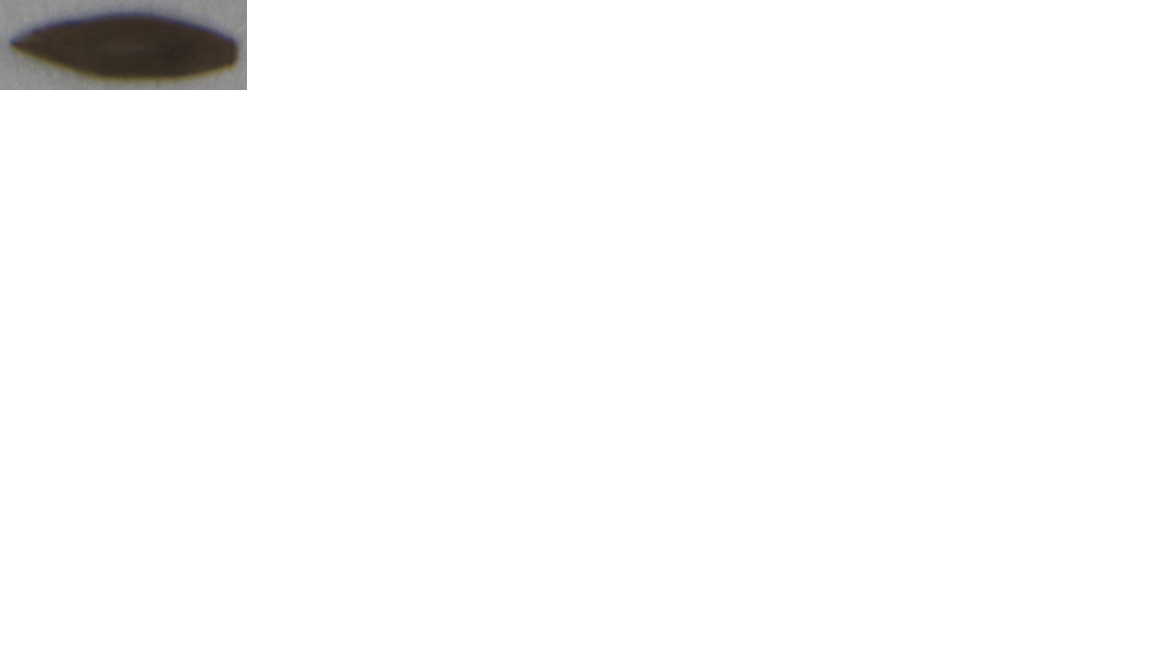
\includegraphics{seed.png}
	\caption{Segmented Seed}
\end{figure}

In this term, we have two different datasets: The Existing data: our preliminary set was started with data collected from before. We added onto it and did transformation; The new data: set which will be collected this term. We work on segmentation and transformation.

In order for our team to collect dataset, we started at meeting with client. All sample of seeds (Tall Fescue) are provided by client. When we get enough sample, we plan to start data collection. At very first time, we used camera which is provided by client. We take several pictures of seeds by that camera. And here is an example of those image (The first stage of data collection):

The first stage of data collection used the camera which is not stronger enough. Images of first stage of data collection is good data, but they are not very clear. Training by these seeds may reduce accuracy rate, or we need an additional large sample of seeds to reach the goal accuracy. There is another disadvantage of using the old camera: it takes time to take one photo. The camera is fixed on a metal framework. Whoever works on taking picture, need additional time to fix position of seeds. (As an example, for me (Xiaoyi), it takes 2 hours for 30 pictures.)

Our team discuss about the first stage of data collection, it is not satisfied for our project. We decided to change into second stage of data collection. In the second stage of data collection, we choose different camera, which is currently call cell-phone. According to our research, our phones have very good cameras which can produce clear images for our training. Here is an example of image which takes by my phone:

(The proportion of image has been adjusted to match the size of documentation)

Pictures from the second stage of data collection are clearer than the first stage of data collection. The improvement of image resolution can bring many benefits: first of all, training by clearer seeds can improve the accuracy rate. In these image from second stage of data collection, characteristics of seeds are clearer. In this case, our module can recognize more characteristics from sample seeds.

The second advantage is the second stage greatly improve the speed of collecting data. Because the image’s resolution is improved, we can adjust the focus and size (screen size) of camera. Which means in each image, we can have more seeds than the first stage of data collection. In the second stage of data collection, we were taking less picture, but it does not reduce the total number of seeds.

In our project, we have a requirement of accuracy rate. To reach the goal accuracy rate, we have a minimum requirement of the dataset. Which is about 5000 seeds. The minimum requirement of the dataset, which can be concerned as “we must have”, has been achieved by now. We have existing data from before, which is about 2000 seeds. In this term, we have the requirement of 3000 seeds. In our data collection part, we took 120 images with 25+ seeds in each image. We hit the minimum requirement, and will do additional data collection to improve the accuracy rate. Our team perfects 200 image as new data this term, it is not a requirement for our goal but an improvement for our project, which means if we have enough time we will finish it.

Our team has reached the goal of minimum requirement of data collection for training. But there is additional part of our seed sample. After we finish the training, we shall start the early module testing. One of my research shows that we should use different sample of seeds to do testing. In the early module testing, we shall try three different ways:

1.	Pre-analysis without classification: in this part, we shall test our module with our training sample, which means the sample we test is from the training dataset. In this test, the result should have a high accuracy rate. This testing method’s result will not be shown up in our final result, it is a warm up testing method, and it is not necessary for our project. If we finish our training early, this method will be applied to our module. Our samples which were used in data collection and training have been kept for this method even we may not use it.
2.	Pre-analysis and classification: in this part, we shall test our module with clean sample. The clean sample means the seeds samples have not been used, for both training and testing. After data collection (include additional data collection in the future), we will have many seeds left. In this testing method, we should use those clean sample for testing. The result of testing may be a little bit lower than the first one. But different with the first testing, this one is required testing which should be applied for both early and later module testing method. In this testing method, only Tall Fescue will be tested. So, the output result of this testing should also be in a high level.
3.	Mixed model testing: this part is a real-environment testing. Off-type seeds will be applied, but in this testing, we shall also be applied both clean seeds and used seeds. Be careful, this testing is still early module test. So, its result should not be concerned as final result.

In conclusion of data collection, our group has finished the requirement of minimum seeds dataset, we will collect additional data later this term.


\section{Data Preparation - Vinayaka Thompson}
So far, the image cleaning part of the project has been going slow. As none of our group members knew how to do image processing we have been trying to figure this out from the ground up. Thus, progress has been slow. During week one and two we were primarily doing research to determine how to go about programming the image splitting / cleaning system. Week 3-4 we started work on the image splitting system. The first week we ended up doing nothing but figuring out how to import the pictures and set up OpenCV to work correctly. We set up OpenCV3.4.0 as that was the current build and the Jetson was on 3.3 from what we read there was no great difference between the two for the applications we were using it for (with the exception of Nvidia’s changes to the jetpack version of OpenCV). Week 4 we started work on the splitting system and have managed to split an image into two different pictures. Week 5 the we had midterms and no significant progress was made and during week6 we have been working on finding critical points to let us split the image on the seeds. Work is still ongoing in trying to reliably detect the seeds. 
Through our struggles with OpenCV there has been one good side effect. We through virtue of not knowing what we are doing have stumbled into some interesting methods for cleaning the picture for use in deep learning. The simple method involves changing the saturation of certain colors to make features pop. The other method involves running the image through a function that extracts the lines. We think that this one might simplify the image for the deep learning algorithm. We have yet to put together a formal test however talking together the logic seems sound. 
Problems impeding progress 
Our progress has been littered with problems. Most of our progress so far has been dealing with the problems we have found.  As was previously mentioned we have little technical knowledge when It comes to computer vision. Thus, the biggest hindrance to our success has been the fact that we must figure out things from the ground up. This means it takes us longer to make systems that might have been trivial, had we someone with knowledge in that area. At the start of term, we thought the image collection system would be complete over winter break and into the first week of term. It quickly became apparent that this would not be the case. To deal with this issue we split the production of the system onto image collection image cleaning /splitting and into machine learning. This made it hard to complete the splitting system the way we had originally planned. The original plan called for the use of the Vision Works/OpenCV libraries found in the NVidia jetpack. This plan was deemed infeasible as when developing the system concurrently the deep learning part had more need for the Jetson than the splitting system. To remedy this issue, we decided to use OpenCV on a Linux device to develop the splitting and cleaning parts of the system. In this case we decided to use a raspberry pi belonging to team member Vinayaka Thompson. The idea being that the pi would simulate the end environment (the Nvidia Terga) well enough to make the port from the pi to the Jetson trivial. This allowed us to develop the systems concurrently potentially reducing the development time by making sure the splitting system is not a bottle neck. This however does not let us optimize the image cleaning and splitting code for the device we will be running it on. We believed this was an acceptable tradeoff so that we could be working on more than one part of the project at the same time. This division was made based on the Clients desire that we stress the accuracy of the system over all other requirements. We felt to do that best we had to get started on the deep learning algorithm. This was the best method we could see. To 
that end we believe that by splitting the work like this we optimize our chance at getting the best accuracy possible through letting our deep learning team work on the Jetson for as long as possible. 
In addition to this problem our team member working on image splitting came down with Pertussis (Whooping Cough) which though not serious enough to stop work it did slow things down as late work nights were often cut short due to coughing and fatigue. Though originally ignored as it was assumed to be a bad cold he has since seen a doctor and been given medication to help reduce the problems. 
Compounding the above two problems, the image splitting/cleaning team has had to deal with running into many dead ends when researching methods of programming with OpenCV. We have been having trouble finding documentation or examples for OpenCV 3.x as most of the examples are produced using opencv2.X Due to the nature of the NVidia jetpack using OpenCV 3.x we are forced to use 3.x so it can be ported to the Jetson with ease. We have not yet found a solution other than keep researching. 
What is left to do Image cleaning 
As a side effect of trying to learn OpenCV we have learned many possible ways we may be able to clean the image. The most interesting involves using a threshold system of sorts to reduce the picture of the seeds to lines. This could help us enhance features of the seed to give the learning algorithm more to work with or it could be used to simplify the image reducing noise and unimportant detail. This simplification might make the image less chaotic for the deep learning algorithm. In addition, we can change to black and white or mess with the intensity of color values to make details stand out more. At this point we need to test these ideas out with the deep learning system to see if any of them provide a real benefit. However, this knowledge opens possibility’s we were not considering at the start of the project. 
What is left to do image splitting 
For image splitting there is one big hurdle left to jump. So far, we have the basics of splitting an image down. We have also discovered how to rotate the area we are taking when splitting the image. This allows us to compensate for the seeds not being straight up and down. However, the big problem left is trying to detect the individual seeds so that we get exactly one image of each seed. 

\section{Training - Omar Elgebaly}
I have been working on primarily on training two models: Naive-bayes and Tensorflow Inception Model with Keras. As of now, I have trained a total of 2,000 Tall Fescue images on the Naive Bayes algorithm. This part was tricky because we are dealing primarily with image data but the Naive Bayes algorithm operates optimally in image recognition scenarios when you output the pixel data into a csv file. I was able to do this through the help of a poster on Quora who provided the following code: \begin{lstlisting}

#!/usr/bin/env python

from __future__ import with_statement
from PIL import Image

im = Image.open('Pictures/300x300.png') #relative path to file

#load the pixel info
pix = im.load()

#get a tuple of the x and y dimensions of the image
width, height = im.size

#open a file to write the pixel data
with open('output_file.csv', 'w+') as f:
f.write('R,G,B\n')

#read the details of each pixel and write them to the file
for x in range(width):
for y in range(height):
r = pix[x,y][0]
g = pix[x,x][1]
b = pix[x,x][2]
f.write('{0},{1},{2}\n'.format(r,g,b))
}    
}
\end{lstlisting}
This code will utilize a Python library called pillow to load and write the pixel info into a .csv file. The next step was to run the Python script for the Naive Baye's Algorithm  \begin{lstlisting}
#source: machinelearningmastery.com
#requires we load image dataset into csv file 
import csv
import random
import math


#load data from CSV file 
def loadCsv(filename): 

lines = csv.reader(open(filename, "rb"))
dataset = list(lines)
for i in range(len(dataset)):
dataset[i] = [float(x) for x in dataset[i]]
return dataset

#split data into training and test sets
def splitDataset(dataset, splitRatio):
trainSize = int(len(dataset) * splitRatio)
trainSet = []
copy = list(dataset)
while len(trainSet) < trainSize:
index = random.randrange(len(copy))
trainSet.append(copy.pop(index))
return [trainSet, copy]

#separate training data instances by class value
def separateByClass(dataset):
separated = {}
for i in range(len(dataset)):
vector = dataset[i]
if (vector[-1] not in separated):
separated[vector[-1]] = []
separated[vector[-1]].append(vector)
return separated

def mean(numbers):
return sum(numbers)/float(len(numbers))

def stdev(numbers):
avg = mean(numbers)
variance = sum([pow(x-avg,2) for x in numbers])/float(len(numbers)-1)
return math.sqrt(variance)

#use zip function to summarize the data by calculating mean and standard deviation of each attribute
def summarize(dataset):
summaries = [(mean(attribute), stdev(attribute)) for attribute in zip(*dataset)]
del summaries[-1]
return summaries

#separate training data into instances grouped by class and calculate summaries for each attribute	
def summarizeByClass(dataset):
separated = separateByClass(dataset)
summaries = {}
for classValue, instances in separated.iteritems():
summaries[classValue] = summarize(instances)
return summaries

##output probability of belonging to a class
def calculateProbability(x, mean, stdev):
exponent = math.exp(-(math.pow(x-mean,2)/(2*math.pow(stdev,2))))
return (1 / (math.sqrt(2*math.pi) * stdev)) * exponent

##calculate probability of a given data instance by multiplying attribute probability for each class. output is a map of class values to probabilities.
def calculateClassProbabilities(summaries, inputVector):
probabilities = {}
for classValue, classSummaries in summaries.iteritems():
probabilities[classValue] = 1
for i in range(len(classSummaries)):
mean, stdev = classSummaries[i]
x = inputVector[i]
probabilities[classValue] *= calculateProbability(x, mean, stdev)
return probabilities

#look for largest probability and return associated class
def predict(summaries, inputVector):
probabilities = calculateClassProbabilities(summaries, inputVector)
bestLabel, bestProb = None, -1
for classValue, probability in probabilities.iteritems():
if bestLabel is None or probability > bestProb:
bestProb = probability
bestLabel = classValue
return bestLabel

#will return a list of predictions for each test instance 	\
def getPredictions(summaries, testSet):
predictions = []
for i in range(len(testSet)):
result = predict(summaries, testSet[i])
predictions.append(result)
return predictions

#will calculate accuracy ration between the class values in the test dataset 
def getAccuracy(testSet, predictions):
correct = 0
for i in range(len(testSet)):
if testSet[i][-1] == predictions[i]:
correct += 1
return (correct/float(len(testSet))) * 100.0

def main():
filename = ''
splitRatio = 0.67
dataset = loadCsv(filename)
trainingSet, testSet = splitDataset(dataset, splitRatio)
print('Split {0} rows into train={1} and test={2} rows').format(len(dataset), len(trainingSet), len(testSet))
# prepare model
summaries = summarizeByClass(trainingSet)
# test model
predictions = getPredictions(summaries, testSet)
accuracy = getAccuracy(testSet, predictions)
print('Accuracy: {0}%').format(accuracy)
\end{lstlisting}
As you can see, the code essentially goes through 6 different steps. It will first load the pixel data from the CSV file. Next, it will split the data into a training set and a testing set. Next, it will categorize training data instances by class value. This allows us to calculate statisitics for each class. As of now, it has only been implemented for Tall Fescue seeds but implementing it for Perennial Ryegrass will be relatively trivial. After that, the data for each class is summarized by calculating the mean and standard deviation of each attribute. Once that is done, it will look for the probability of data instance belonging to a class value. When that has finished, the model will make predictions for each data instance and return a list of predictions. These predictions will then be compared to the class values in the test dataset and output the accuracy of the model in a percentage.

The linear model is a good first step for this project but the ultimate goal is deep learning. So far, I have been running into issues with setting up Tensorflow to use the CUDA enabled GPU. I noticed it was taking incredibly long to train a small dataset. I realized it was because I built the Tensorflow wheel without CUDA. It also took some time to figure out that the Jettson TX2 does not come with Jetpack 3.0 installed. Instead, you must download it from the website and flash it on a 64-bit Linux 14.04 host machine and then load it onto the Jettson via the provided micro USB to USB connection. I also ran into some issues with Bazel. More specifically, it seems as if Bazel bugs out and does not see my JAVA\_HOME environment variable when I use OpenJDK 1.8. Even more strangely, it works with the previous version, which is 1.7. 

Since writing our design doc, we have decided to use multiple models for this project. As of now, I only have plans to implement the Naive-Bayes and Tensorflow models but I will move onto others if time constraints allow for it. I have discussed with both the client and the TA that doing a comparison on the accuracy of different models in identifying seeds is a good way to learn more about which models are best for image recognition. It is a neat little side project that may be valuable to future developers who pursue this line of work.

The next steps in this project for me are to add images of Perennial Ryegrass to the training set for the Naive-Bayes model. Additionally, I now have Jetpack set up on the Jettson TX2 and have figured out a way to get Tensorflow 1.5, which is compatible with our version of CUDA and CUDN. I will then train a neural net that will use the GPU for computing power on images of Tall Fescue and Perennial Ryegrass. This will be the top priority as this is the core functionality of the product we are producing. As of now we have about 2000 images for Tall Fescue and Perennial Ryegrass that are processed and ready to train. We will continue collecting more data and training to continuously improve our accuracy and learning rate. Our initial goal is 75\% accuracy but will strive for 80\%. We also plan on exploring other models potentially over spring break as we believe it is a nice side project to compare different models. It would also fit into our poster nicely.

\section{Conclusion}
So far, our progress this term has been moving slowly but steadily. We have resolved a lot of our communication issues through use of the instant message voice over IP app Discord. We have a very preliminary model trained as of now but that is meant as more of a test of our image quality more than anything. We figured it would be smart to see if a simple model can be trained on the images we have before pursuing it more aggressively with deep learning. Data collection and processing is an ongoing process so we Xiaoyi and Vinayaka will continue working on those parts. I will continue working on the linear model and the deep learning model. If we get the deep learning model working adequately, we plan to explore different models. This will allow all group members to become familiar with how training works.

\end{document}





